
\subsection{Repräsentationen}
\label{representations}
\subsubsection{Autoencoder}

\emph{Feedforward}-Netzwerk, das darauf trainiert wird, die Eingabe zur Ausgabe zu kopieren. Kodierer und Dekodierer sind antisymmetrisch aufgebaut (Anzahl der Eingabeneuronen im Kodierer entspricht Anzahl der Ausgabeneuronen im Dekodierer). Die dazwischen liegende Schicht heißt \emph{Flaschenhals}, wenn der Autoencoder \emph{undercomplete}, d.h. $\hat{n}<n$ ist.\\

\begin{figure}[H]
    \centering
    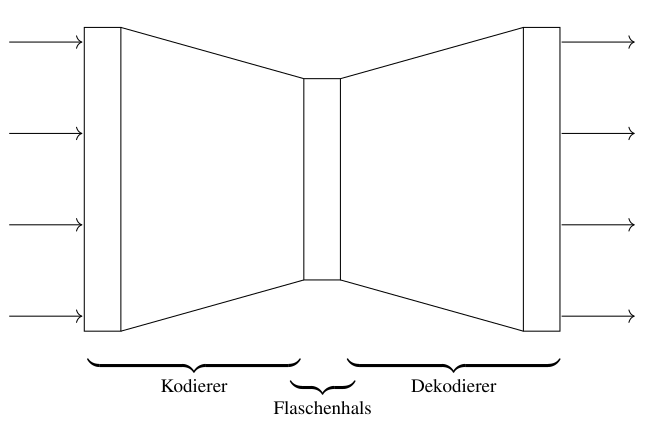
\includegraphics[width=0.5\textwidth]{deepLearning/autoencoder.png}
    \caption{Autoencoder}
\end{figure}

\underline{\textbf{Kompression}}: Kodierer mit Funktion $f$ und Dekodierer mit Funktion $g$ so trainieren, dass der Flaschenhals (undercomplete Autoencoder mit $\hat{n}<n$) $g\circ f$ einen Wert $x_i$ möglichst Verlustfrei wieder ausgibt. Kodierer wird dabei genutzt Daten zu komprimieren, Dekodierer um Daten zu dekomprimieren. Sind alle Aktiierungsfunktionen linear, hat der Autoencoder die gleiche Kompressionsstruktur wie bei der PCA.\\

\underline{\textbf{Sparse Autoencoder (SAE)}}: Flaschenhals hat $\hat{n}>n$ und ist damit overcomplete $\rightarrow$ kann z.B. eingesetzt werden, um Ausgabe besser zu generalisieren. Damit potentiell alle Neuronen im Flaschenhals überhaupt genutzt werden, wird ein Regulatisierungsparameter $\lambda$ in der Loss-Funktion eingeführt ($L^\text{sae}(D, g\circ f)=L^\text{auto}(D, g\circ f)+\lambda\sum_{i=1}^{m}\Vert f(x^{(i)})\Vert$)\\

\underline{\textbf{Denoising Auto Encoder (DAE)}}: Autoencoder wird mit verrauschten Eingabedaten trainiert (Erzeugt zB. durch Gauss), um die ursprünglichen Daten wiederherzustellen $\rightarrow$ Auch: Datengenerierung als wichtige Ausgabe.\\


\subsubsection{Generative Adversial Networks (GANs)}

GANs bestehen aus zwei separaten \emph{Feedforward}-Netzwerken: Einem \emph{Generator} und einem \emph{Diskriminator}. Der Generator erzeugt Daten (z.B. Bilder), die dem Diskriminator vorgelegt werden. Der Diskriminator versucht zu entscheiden, ob die Daten vom Generator oder aus dem Trainingsdatensatz stammen. Der Generator wird trainiert, um den Diskriminator zu täuschen, während der Diskriminator trainiert wird, um den Generator zu entlarven.\\

\begin{figure}[H]
    \centering
    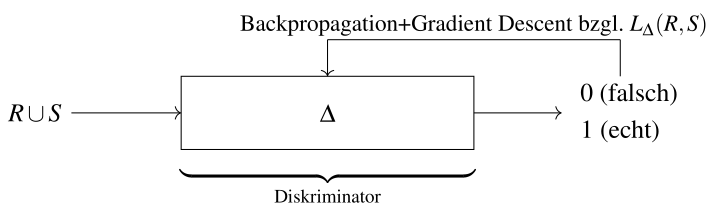
\includegraphics[width=0.5\textwidth]{deepLearning/discriminator.png}
    \caption{Lernschritt eines Diskriminators}
\end{figure}

\begin{figure}[H]
    \centering
    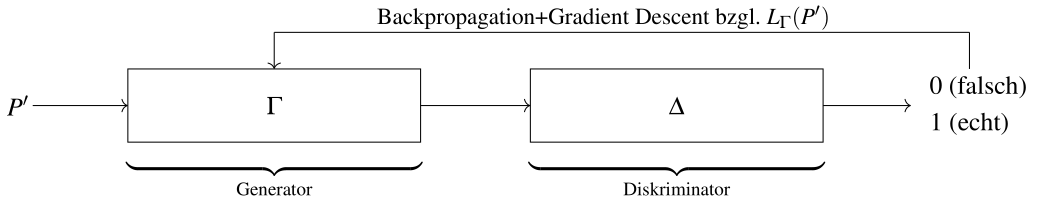
\includegraphics[width=0.5\textwidth]{deepLearning/generator.png}
    \caption{Lernschritt eines Generators}
\end{figure}

Wichtig: Beim Lernschritt des Generators durchläuft der Backpropagation-Algorithmus auch den Diskriminator, passt dort jedoch keine Gewichte an.\\